% Options for packages loaded elsewhere
% Options for packages loaded elsewhere
\PassOptionsToPackage{unicode}{hyperref}
\PassOptionsToPackage{hyphens}{url}
\PassOptionsToPackage{dvipsnames,svgnames,x11names}{xcolor}
%
\documentclass[
  letterpaper,
  DIV=11,
  numbers=noendperiod]{scrreprt}
\usepackage{xcolor}
\usepackage{amsmath,amssymb}
\setcounter{secnumdepth}{5}
\usepackage{iftex}
\ifPDFTeX
  \usepackage[T1]{fontenc}
  \usepackage[utf8]{inputenc}
  \usepackage{textcomp} % provide euro and other symbols
\else % if luatex or xetex
  \usepackage{unicode-math} % this also loads fontspec
  \defaultfontfeatures{Scale=MatchLowercase}
  \defaultfontfeatures[\rmfamily]{Ligatures=TeX,Scale=1}
\fi
\usepackage{lmodern}
\ifPDFTeX\else
  % xetex/luatex font selection
\fi
% Use upquote if available, for straight quotes in verbatim environments
\IfFileExists{upquote.sty}{\usepackage{upquote}}{}
\IfFileExists{microtype.sty}{% use microtype if available
  \usepackage[]{microtype}
  \UseMicrotypeSet[protrusion]{basicmath} % disable protrusion for tt fonts
}{}
\makeatletter
\@ifundefined{KOMAClassName}{% if non-KOMA class
  \IfFileExists{parskip.sty}{%
    \usepackage{parskip}
  }{% else
    \setlength{\parindent}{0pt}
    \setlength{\parskip}{6pt plus 2pt minus 1pt}}
}{% if KOMA class
  \KOMAoptions{parskip=half}}
\makeatother
% Make \paragraph and \subparagraph free-standing
\makeatletter
\ifx\paragraph\undefined\else
  \let\oldparagraph\paragraph
  \renewcommand{\paragraph}{
    \@ifstar
      \xxxParagraphStar
      \xxxParagraphNoStar
  }
  \newcommand{\xxxParagraphStar}[1]{\oldparagraph*{#1}\mbox{}}
  \newcommand{\xxxParagraphNoStar}[1]{\oldparagraph{#1}\mbox{}}
\fi
\ifx\subparagraph\undefined\else
  \let\oldsubparagraph\subparagraph
  \renewcommand{\subparagraph}{
    \@ifstar
      \xxxSubParagraphStar
      \xxxSubParagraphNoStar
  }
  \newcommand{\xxxSubParagraphStar}[1]{\oldsubparagraph*{#1}\mbox{}}
  \newcommand{\xxxSubParagraphNoStar}[1]{\oldsubparagraph{#1}\mbox{}}
\fi
\makeatother

\usepackage{color}
\usepackage{fancyvrb}
\newcommand{\VerbBar}{|}
\newcommand{\VERB}{\Verb[commandchars=\\\{\}]}
\DefineVerbatimEnvironment{Highlighting}{Verbatim}{commandchars=\\\{\}}
% Add ',fontsize=\small' for more characters per line
\usepackage{framed}
\definecolor{shadecolor}{RGB}{241,243,245}
\newenvironment{Shaded}{\begin{snugshade}}{\end{snugshade}}
\newcommand{\AlertTok}[1]{\textcolor[rgb]{0.68,0.00,0.00}{#1}}
\newcommand{\AnnotationTok}[1]{\textcolor[rgb]{0.37,0.37,0.37}{#1}}
\newcommand{\AttributeTok}[1]{\textcolor[rgb]{0.40,0.45,0.13}{#1}}
\newcommand{\BaseNTok}[1]{\textcolor[rgb]{0.68,0.00,0.00}{#1}}
\newcommand{\BuiltInTok}[1]{\textcolor[rgb]{0.00,0.23,0.31}{#1}}
\newcommand{\CharTok}[1]{\textcolor[rgb]{0.13,0.47,0.30}{#1}}
\newcommand{\CommentTok}[1]{\textcolor[rgb]{0.37,0.37,0.37}{#1}}
\newcommand{\CommentVarTok}[1]{\textcolor[rgb]{0.37,0.37,0.37}{\textit{#1}}}
\newcommand{\ConstantTok}[1]{\textcolor[rgb]{0.56,0.35,0.01}{#1}}
\newcommand{\ControlFlowTok}[1]{\textcolor[rgb]{0.00,0.23,0.31}{\textbf{#1}}}
\newcommand{\DataTypeTok}[1]{\textcolor[rgb]{0.68,0.00,0.00}{#1}}
\newcommand{\DecValTok}[1]{\textcolor[rgb]{0.68,0.00,0.00}{#1}}
\newcommand{\DocumentationTok}[1]{\textcolor[rgb]{0.37,0.37,0.37}{\textit{#1}}}
\newcommand{\ErrorTok}[1]{\textcolor[rgb]{0.68,0.00,0.00}{#1}}
\newcommand{\ExtensionTok}[1]{\textcolor[rgb]{0.00,0.23,0.31}{#1}}
\newcommand{\FloatTok}[1]{\textcolor[rgb]{0.68,0.00,0.00}{#1}}
\newcommand{\FunctionTok}[1]{\textcolor[rgb]{0.28,0.35,0.67}{#1}}
\newcommand{\ImportTok}[1]{\textcolor[rgb]{0.00,0.46,0.62}{#1}}
\newcommand{\InformationTok}[1]{\textcolor[rgb]{0.37,0.37,0.37}{#1}}
\newcommand{\KeywordTok}[1]{\textcolor[rgb]{0.00,0.23,0.31}{\textbf{#1}}}
\newcommand{\NormalTok}[1]{\textcolor[rgb]{0.00,0.23,0.31}{#1}}
\newcommand{\OperatorTok}[1]{\textcolor[rgb]{0.37,0.37,0.37}{#1}}
\newcommand{\OtherTok}[1]{\textcolor[rgb]{0.00,0.23,0.31}{#1}}
\newcommand{\PreprocessorTok}[1]{\textcolor[rgb]{0.68,0.00,0.00}{#1}}
\newcommand{\RegionMarkerTok}[1]{\textcolor[rgb]{0.00,0.23,0.31}{#1}}
\newcommand{\SpecialCharTok}[1]{\textcolor[rgb]{0.37,0.37,0.37}{#1}}
\newcommand{\SpecialStringTok}[1]{\textcolor[rgb]{0.13,0.47,0.30}{#1}}
\newcommand{\StringTok}[1]{\textcolor[rgb]{0.13,0.47,0.30}{#1}}
\newcommand{\VariableTok}[1]{\textcolor[rgb]{0.07,0.07,0.07}{#1}}
\newcommand{\VerbatimStringTok}[1]{\textcolor[rgb]{0.13,0.47,0.30}{#1}}
\newcommand{\WarningTok}[1]{\textcolor[rgb]{0.37,0.37,0.37}{\textit{#1}}}

\usepackage{longtable,booktabs,array}
\usepackage{calc} % for calculating minipage widths
% Correct order of tables after \paragraph or \subparagraph
\usepackage{etoolbox}
\makeatletter
\patchcmd\longtable{\par}{\if@noskipsec\mbox{}\fi\par}{}{}
\makeatother
% Allow footnotes in longtable head/foot
\IfFileExists{footnotehyper.sty}{\usepackage{footnotehyper}}{\usepackage{footnote}}
\makesavenoteenv{longtable}
\usepackage{graphicx}
\makeatletter
\newsavebox\pandoc@box
\newcommand*\pandocbounded[1]{% scales image to fit in text height/width
  \sbox\pandoc@box{#1}%
  \Gscale@div\@tempa{\textheight}{\dimexpr\ht\pandoc@box+\dp\pandoc@box\relax}%
  \Gscale@div\@tempb{\linewidth}{\wd\pandoc@box}%
  \ifdim\@tempb\p@<\@tempa\p@\let\@tempa\@tempb\fi% select the smaller of both
  \ifdim\@tempa\p@<\p@\scalebox{\@tempa}{\usebox\pandoc@box}%
  \else\usebox{\pandoc@box}%
  \fi%
}
% Set default figure placement to htbp
\def\fps@figure{htbp}
\makeatother





\setlength{\emergencystretch}{3em} % prevent overfull lines

\providecommand{\tightlist}{%
  \setlength{\itemsep}{0pt}\setlength{\parskip}{0pt}}



 


\KOMAoption{captions}{tableheading}
\makeatletter
\@ifpackageloaded{tcolorbox}{}{\usepackage[skins,breakable]{tcolorbox}}
\@ifpackageloaded{fontawesome5}{}{\usepackage{fontawesome5}}
\definecolor{quarto-callout-color}{HTML}{909090}
\definecolor{quarto-callout-note-color}{HTML}{0758E5}
\definecolor{quarto-callout-important-color}{HTML}{CC1914}
\definecolor{quarto-callout-warning-color}{HTML}{EB9113}
\definecolor{quarto-callout-tip-color}{HTML}{00A047}
\definecolor{quarto-callout-caution-color}{HTML}{FC5300}
\definecolor{quarto-callout-color-frame}{HTML}{acacac}
\definecolor{quarto-callout-note-color-frame}{HTML}{4582ec}
\definecolor{quarto-callout-important-color-frame}{HTML}{d9534f}
\definecolor{quarto-callout-warning-color-frame}{HTML}{f0ad4e}
\definecolor{quarto-callout-tip-color-frame}{HTML}{02b875}
\definecolor{quarto-callout-caution-color-frame}{HTML}{fd7e14}
\makeatother
\makeatletter
\@ifpackageloaded{bookmark}{}{\usepackage{bookmark}}
\makeatother
\makeatletter
\@ifpackageloaded{caption}{}{\usepackage{caption}}
\AtBeginDocument{%
\ifdefined\contentsname
  \renewcommand*\contentsname{Table of contents}
\else
  \newcommand\contentsname{Table of contents}
\fi
\ifdefined\listfigurename
  \renewcommand*\listfigurename{List of Figures}
\else
  \newcommand\listfigurename{List of Figures}
\fi
\ifdefined\listtablename
  \renewcommand*\listtablename{List of Tables}
\else
  \newcommand\listtablename{List of Tables}
\fi
\ifdefined\figurename
  \renewcommand*\figurename{Figure}
\else
  \newcommand\figurename{Figure}
\fi
\ifdefined\tablename
  \renewcommand*\tablename{Table}
\else
  \newcommand\tablename{Table}
\fi
}
\@ifpackageloaded{float}{}{\usepackage{float}}
\floatstyle{ruled}
\@ifundefined{c@chapter}{\newfloat{codelisting}{h}{lop}}{\newfloat{codelisting}{h}{lop}[chapter]}
\floatname{codelisting}{Listing}
\newcommand*\listoflistings{\listof{codelisting}{List of Listings}}
\makeatother
\makeatletter
\makeatother
\makeatletter
\@ifpackageloaded{caption}{}{\usepackage{caption}}
\@ifpackageloaded{subcaption}{}{\usepackage{subcaption}}
\makeatother
\usepackage{bookmark}
\IfFileExists{xurl.sty}{\usepackage{xurl}}{} % add URL line breaks if available
\urlstyle{same}
\hypersetup{
  pdftitle={E資格 レベルアップ問題集},
  pdfauthor={IRIE NORIFUMI},
  colorlinks=true,
  linkcolor={blue},
  filecolor={Maroon},
  citecolor={Blue},
  urlcolor={Blue},
  pdfcreator={LaTeX via pandoc}}


\title{E資格 レベルアップ問題集}
\author{IRIE NORIFUMI}
\date{}
\begin{document}
\maketitle

\renewcommand*\contentsname{Table of contents}
{
\hypersetup{linkcolor=}
\setcounter{tocdepth}{2}
\tableofcontents
}

\bookmarksetup{startatroot}

\chapter*{前書き}\label{ux524dux66f8ux304d}
\addcontentsline{toc}{chapter}{前書き}

\markboth{前書き}{前書き}

本問題集では日本ディープラーニング協会(JDLA)が実施する「E資格」に向け、E2024\#2のシラバスに沿った問題を掲載しています。\\
暗記で解ける問題というよりは数学的・論理的背景を問うような問題になるよう心がけて作成しています。\\
個人的にE資格は統計検定2級以上・準1級以下のレベルである印象です。準1級に苦戦している方は息抜きに受けてみるといいかもしれません。\\
他にも、E資格が受かるレベルになると、GPT5などの最新モデルの発表があった際に論文やまとめ記事をざっくり読んでその特徴を掴めます。\\
機械学習が必要なくなる時代になっても、他の人よりモデルの特徴を汲んだ上質なプロンプトが書けるかもしれません。

\section*{対象読者}\label{ux5bfeux8c61ux8aadux8005}
\addcontentsline{toc}{section}{対象読者}

\markright{対象読者}

\begin{itemize}
\tightlist
\item
  E資格の受験を予定している方
\item
  統計検定2級でもの足りていない方
\item
  深層学習を実務で使う方
\item
  GPT5などSOTAを達成した最新モデルの背景をより深く理解したい方
\end{itemize}

\begin{center}\rule{0.5\linewidth}{0.5pt}\end{center}

本書が、受験勉強の効率化と深層学習理解の一助となることを願っています。

\bookmarksetup{startatroot}

\chapter{目次}\label{ux76eeux6b21}

本書はE資格のE2024\#2のシラバスに沿った以下の章節で構成しています。\\
解答・解説は「解答一覧」をご覧ください。

\part{2.機械学習(Machine Learning)}

\chapter{1. 機械学習の基礎 (Machine Learning
Basics)}\label{ux6a5fux68b0ux5b66ux7fd2ux306eux57faux790e-machine-learning-basics}

\part{3.深層学習基礎(Basic Deep-learning)}

\chapter{1. 順伝播型ネットワーク (Feedforward Neural
Network)}\label{ux9806ux4f1dux64adux578bux30cdux30c3ux30c8ux30efux30fcux30af-feedforward-neural-network}

\subsection{問1}\label{ux554f1}

以下は2値分類のバイナリクロスエントロピー損失を実装するコードである。空欄(ア)に入る正しいコードを選べ。

\begin{Shaded}
\begin{Highlighting}[]
\ImportTok{import}\NormalTok{ numpy }\ImportTok{as}\NormalTok{ np}

\KeywordTok{def}\NormalTok{ binary\_crossentropy(y\_true, y\_pred):}
    \CommentTok{"""}
\CommentTok{    y\_true: 真のラベル [batch\_size] (0 or 1)}
\CommentTok{    y\_pred: 予測確率 [batch\_size] (0\textasciitilde{}1の値)}
\CommentTok{    """}
    \CommentTok{\# クリッピング}
\NormalTok{    epsilon }\OperatorTok{=} \FloatTok{1e{-}15}
\NormalTok{    y\_pred }\OperatorTok{=}\NormalTok{ (ア)}
    
    \CommentTok{\# バイナリクロスエントロピー計算}
\NormalTok{    loss }\OperatorTok{=} \OperatorTok{{-}}\NormalTok{np.mean(y\_true }\OperatorTok{*}\NormalTok{ np.log(y\_pred) }\OperatorTok{+}\NormalTok{ (}\DecValTok{1} \OperatorTok{{-}}\NormalTok{ y\_true) }\OperatorTok{*}\NormalTok{ np.log(}\DecValTok{1} \OperatorTok{{-}}\NormalTok{ y\_pred))}
    \ControlFlowTok{return}\NormalTok{ loss}
\end{Highlighting}
\end{Shaded}

A. np.clip(y\_pred, epsilon, 1.0)\\
B. np.clip(y\_pred, 0.0, 1 - epsilon)\\
C. np.clip(y\_pred, epsilon, 1 - epsilon)\\
D. np.maximum(y\_pred, epsilon)

\subsection{問2}\label{ux554f2}

以下は多クラス分類のソフトマックス関数を実装するコードである。数値安定性を考慮した空欄(ア)、(イ)に入る正しいコードを選べ。

\begin{Shaded}
\begin{Highlighting}[]
\ImportTok{import}\NormalTok{ numpy }\ImportTok{as}\NormalTok{ np}

\KeywordTok{def}\NormalTok{ softmax(x):}
    \CommentTok{"""}
\CommentTok{    x: ロジット [batch\_size, num\_classes]}
\CommentTok{    """}
    \CommentTok{\# 数値安定性のため最大値を引く}
\NormalTok{    x\_max }\OperatorTok{=}\NormalTok{ (ア)}
\NormalTok{    x\_shifted }\OperatorTok{=}\NormalTok{ x }\OperatorTok{{-}}\NormalTok{ x\_max}
    
    \CommentTok{\# ソフトマックス計算}
\NormalTok{    exp\_x }\OperatorTok{=}\NormalTok{ np.exp(x\_shifted)}
\NormalTok{    sum\_exp }\OperatorTok{=}\NormalTok{ (イ)}
    
    \ControlFlowTok{return}\NormalTok{ exp\_x }\OperatorTok{/}\NormalTok{ sum\_exp}
\end{Highlighting}
\end{Shaded}

A. ア: np.max(x, axis=1, keepdims=True), イ: np.sum(exp\_x, axis=1,
keepdims=True)\\
B. ア: np.max(x, axis=0, keepdims=True), イ: np.sum(exp\_x, axis=0,
keepdims=True)\\
C. ア: np.max(x, axis=1), イ: np.sum(exp\_x, axis=1)\\
D. ア: np.maximum(x, 0), イ: np.sum(exp\_x)

\subsection{問3}\label{ux554f3}

以下のtanh関数のプログラムで空欄(ア)に入るものを選べ。

\begin{Shaded}
\begin{Highlighting}[]
\ImportTok{import}\NormalTok{ numpy }\ImportTok{as}\NormalTok{ np}

\KeywordTok{def}\NormalTok{ tanh(x):}
\NormalTok{    y }\OperatorTok{=}\NormalTok{ (ア)}
    \ControlFlowTok{return}\NormalTok{ y}
\end{Highlighting}
\end{Shaded}

A. (np.exp(x) + np.exp(-x)) / (np.exp(x) + np.exp(-x))\\
B. (np.exp(x) + np.exp(-x)) / (np.exp(x) - np.exp(-x))\\
C. (np.exp(x) -- np.exp(-x)) / (np.exp(x) - np.exp(-x))\\
D. (np.exp(x) -- np.exp(-x)) / (np.exp(x) + np.exp(-x))

\chapter{2. 深層学習のための最適化
(Optimization)}\label{ux6df1ux5c64ux5b66ux7fd2ux306eux305fux3081ux306eux6700ux9069ux5316-optimization}

\subsection{問1}\label{ux554f1-1}

次の計算グラフは、ロジット ( z = {[}z\_1, z\_2, z\_3{]} )
からソフトマックスを計算し、クロスエントロピー損失 ( L )
を求める順伝播を表している。

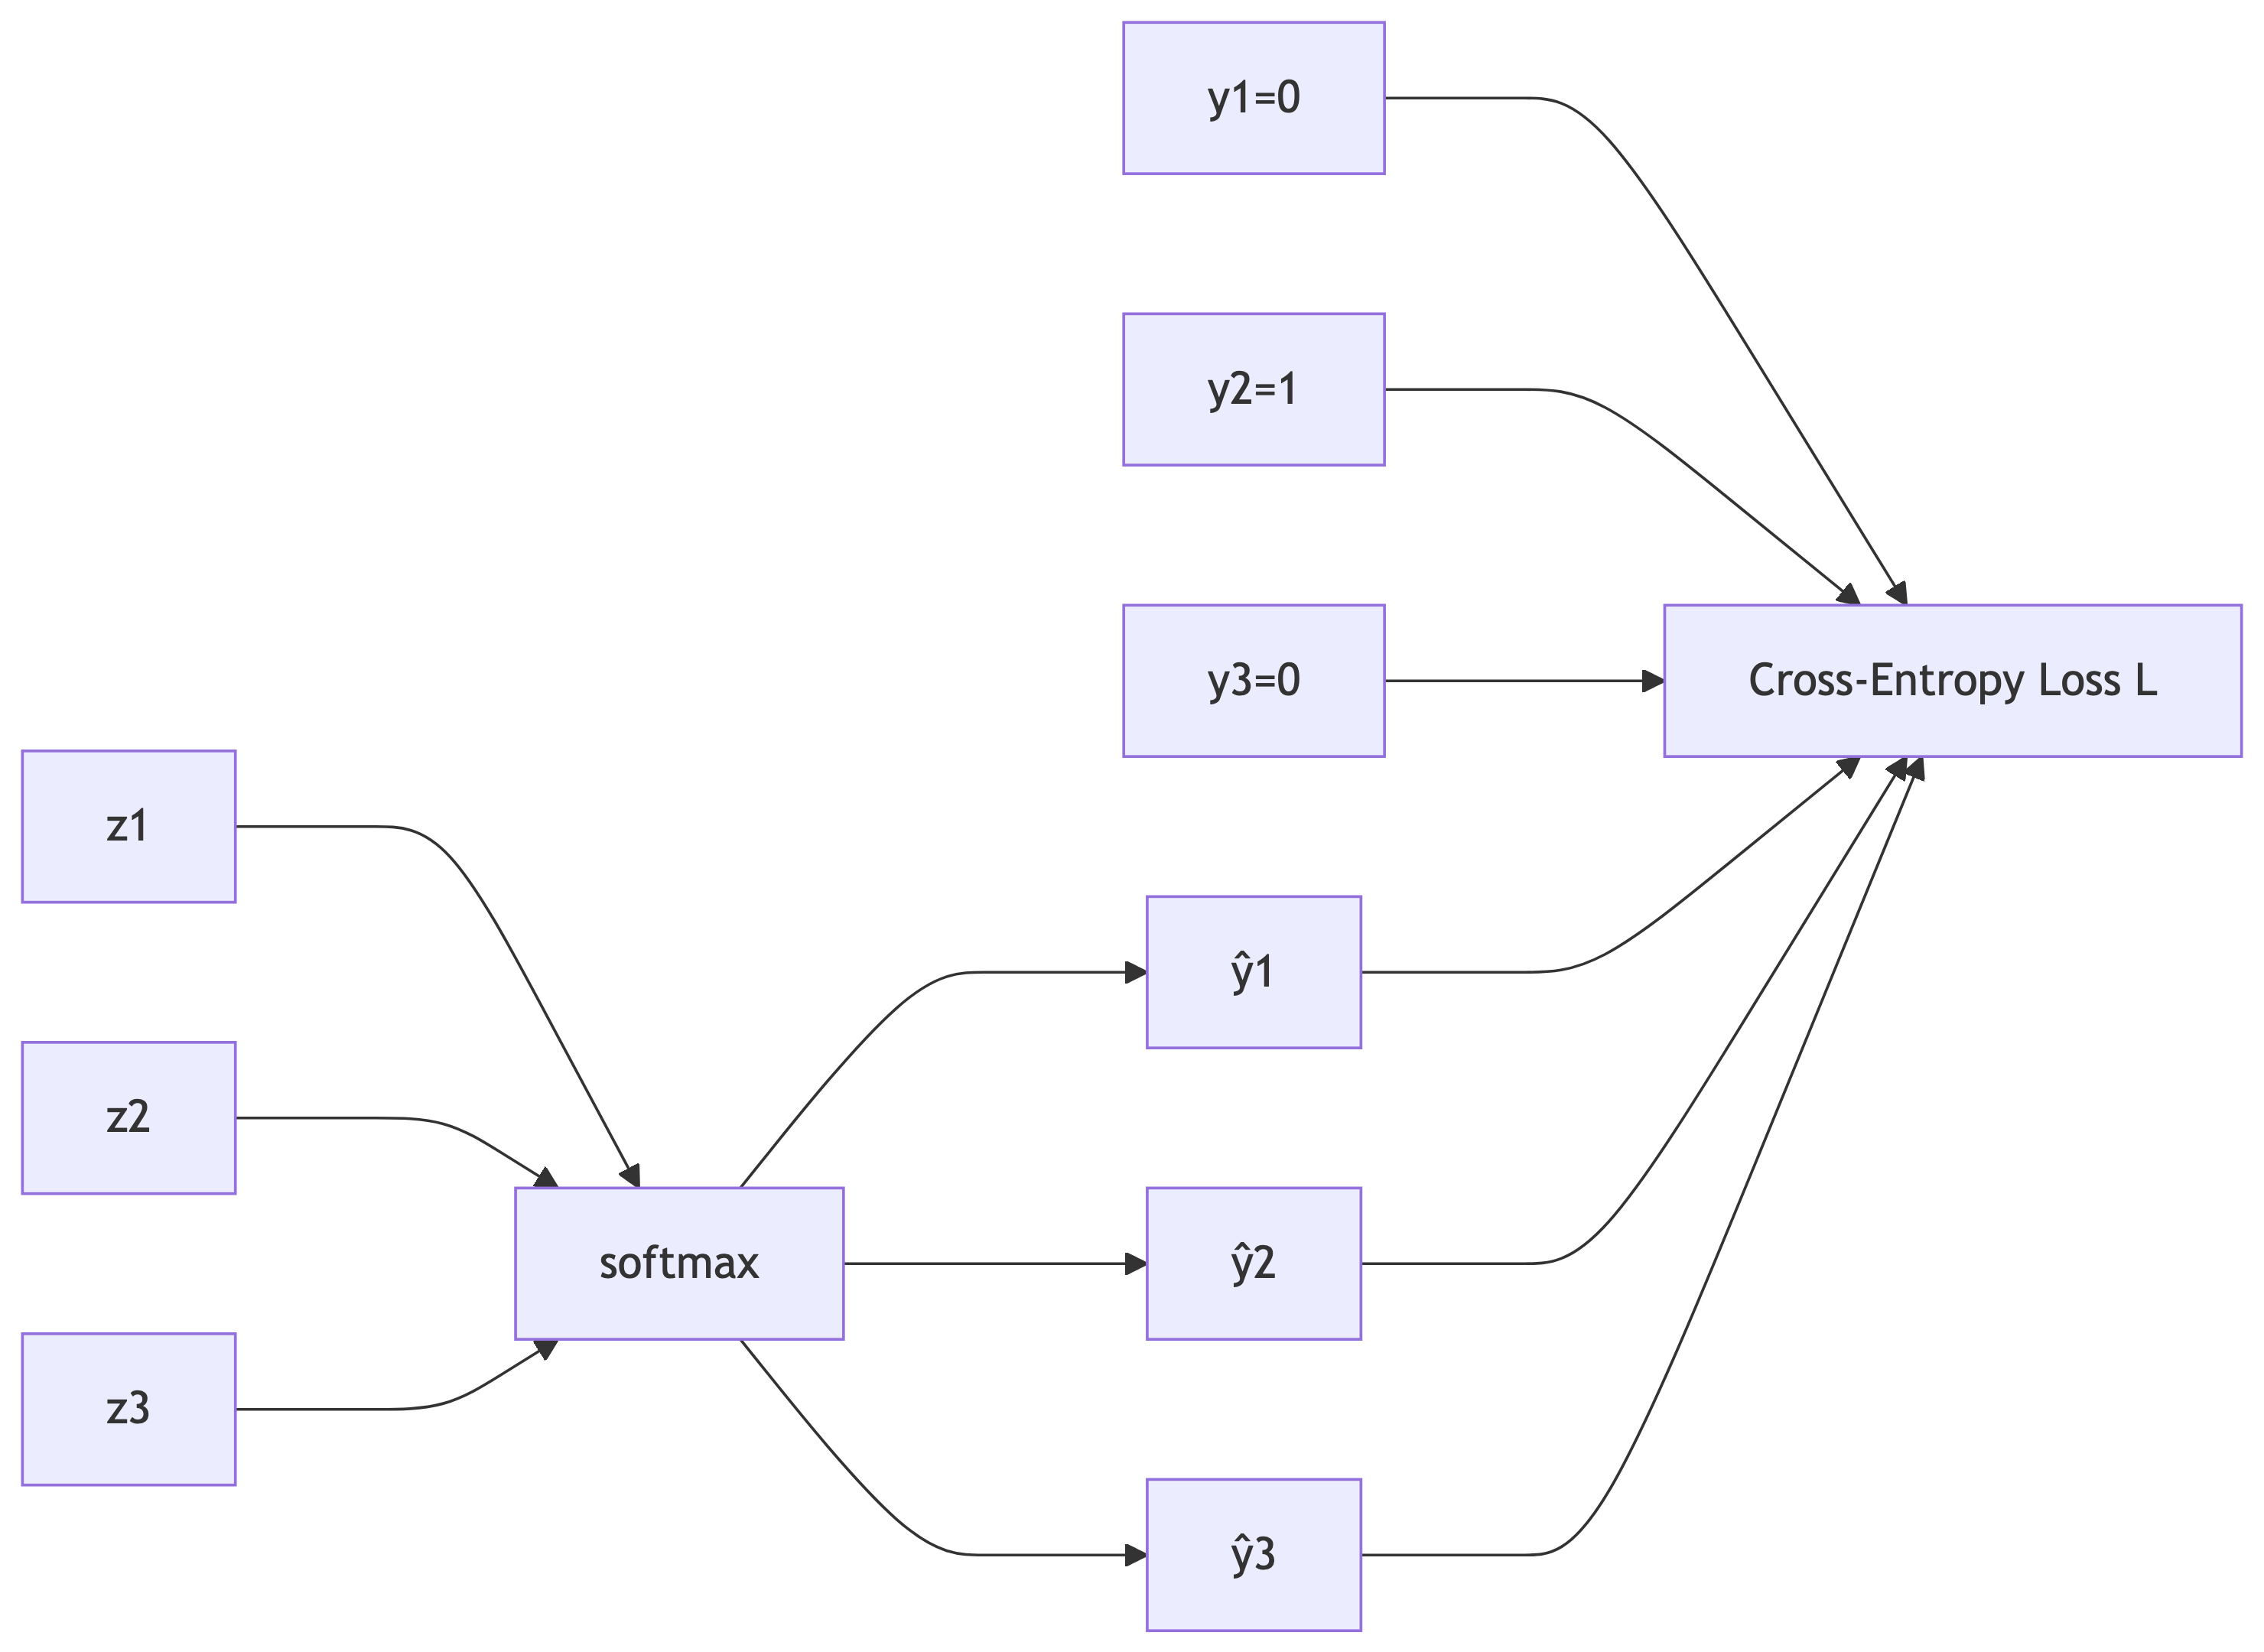
\includegraphics[width=8.42in,height=6.15in]{chapters/part3/02_optimization_files/figure-latex/mermaid-figure-1.png}

I.
逆伝播で\(\frac{∂𝐿}{∂𝑧_j}\)を求めたときの一般公式として正しいものを選べ。\\
ただし、ソフトマックスとクロスエントロピー損失は以下で表せるものとする。

\[
\hat{y}_i = \frac{\exp(z_i)}{\sum_{k} \exp(z_k)}
\]

\[
L = - \sum_{i} y_i \log(\hat{y}_i)
\]

A. \(𝑦_j−\hat{y}_j\)\\
B. \(\hat{y}_j-𝑦_j\)\\
C. \(\frac{-y_j}{\hat{y}_j}\)\\
D. \(\hat{y}_j(1-𝑦_j)\)

II.3クラス分類問題で、真のラベル\(y = [0,1,0]\)、ソフトマックスの出力\(\hat{y}=[0.2, 0.3, 0.5]\)のとき、
\(\frac{∂𝐿}{∂𝑧_2}\)を求めよ。\\
A. -0.7\\
B. 0.7\\
C. -0.3\\
D. 0.3

\subsection{問2}\label{ux554f2-1}

AdaGradアルゴリズムの数式は以下のように表される:

\[
h_t = h_{t-1} + ∇E(W_t) ⊙ ∇E(W_t)
α_t = α_0 × (1/√(h_t + ε))
W_{t+1} = W_t - α_t ⊙ ∇E(W_t)
\]

この数式に関する説明として正しくないものはどれか。

A.
h\_tは各パラメータの累積二乗勾配を表し、そのパラメータがどれだけ激しく更新されてきたかを記録する\\
B.
α\_tは各パラメータごとに適応的に調整される学習率で、累積二乗勾配が大きいほど学習率は小さくなる\\
C.
⊙はアダマール積(要素ごとの積)を表し、各パラメータを独立して扱うために使用される\\
D.
εは数値安定化項で、h\_tが大きくなりすぎて学習率が極端に小さくなることを防ぐ

\chapter{3. 畳み込みニューラルネットワーク (Convolutional
Neural)}\label{ux7573ux307fux8fbcux307fux30cbux30e5ux30fcux30e9ux30ebux30cdux30c3ux30c8ux30efux30fcux30af-convolutional-neural}

\subsection{問1.}\label{ux554f1.}

ある1枚の画像(1チャンネル)に対して、次の条件で im2col 変換を行う。\\
入力画像サイズ:5×5\\
フィルターサイズ:3×3\\
ストライド:1\\
パディング:0

I.
この時、畳み込み演算の出力サイズの公式を用いて、出力の高さと幅を計算せよ。\\
A. (2, 2)\\
B. (3, 3)\\
C. (4, 4)\\
D. (5, 5)

\begin{enumerate}
\def\labelenumi{\Roman{enumi}.}
\setcounter{enumi}{1}
\tightlist
\item
  このとき、im2colによって生成される行列の形状(im\_col.shape)として最も適切なものはどれか。
  ただし、フィルターは1枚であり、チャンネル数は1とする。
\end{enumerate}

A. (3, 3)\\
B. (9, 9)\\
C. (9, 25)\\
D. (3, 9)

\part{第4章.深層学習応用(Advanced Deep-learning)}

\chapter{1. 画像認識(Image
Recognition)}\label{ux753bux50cfux8a8dux8b58image-recognition}

\subsection{問1}\label{ux554f1-2}

Vision Transformer(ViT)の特徴として正しいものを1つ選べ。\\
A.
画像を1ピクセルごとに分割して系列として入力し、CNNよりもパラメータ数が少なくなる傾向がある。\\
B.
画像を固定サイズのパッチに分割し、系列としてTransformerに入力するため、自己注意機構で画像全体の依存関係を学習できる。\\
C.
CNNの畳み込み層を多用するため、自然言語処理タスクへの応用は困難である。\\
D.
入力画像サイズを大きくしてもパラメータ数が比例して増えるため、高解像度画像の学習は計算負荷が低い。

\chapter{2. 物体検出(Object
Detection)}\label{ux7269ux4f53ux691cux51faobject-detection}

\subsection{問1}\label{ux554f1-3}

以下のうち、FCOSについて誤っているものはどれか。\\
A. FCOSはアンカーボックスのサイズ・アスペクト比・数を事前に設定する。\\
B. FCOSはFeature Pyramid
Network(FPN)により生成される複数のサイズの特徴マップを用いて、大小様々な物体を検出できる。\\
C. FCOS
はバウンディングボックスの座標ではなく、各ピクセル座標においてフレームまでの距離を回帰する。\\
D. FCOS
では対象物体の中心から離れた位置に低品質の予測バウンディングボックスが生成されるため、対策としてCenter-nessブランチが導入された。

\subsection{問2}\label{ux554f2-2}

R-CNNの英語名(A)を答えよ。
また、この名称の由来となったROIに関して、ROIを見つけ出すアルゴリズムの総称(B)と、R-CNNにおけるアルゴリズムの手法(C)を答えよ。

\chapter{3. Semantic Segmentation (Semantic
Segmentation)}\label{semantic-segmentation-semantic-segmentation}

\subsection{問1}\label{ux554f1-4}

FCN(Fully Convolutional
Network)は、画像のセマンティックセグメンテーションのために設計されたネットワークであり、全結合層の代わりに(あ)を用いて、入力画像と同じ空間解像度の出力を得ることが可能である。また、分類タスクで用いられる典型的なCNN(例:VGG,
ResNet)をベースとして、出力特徴マップを元の画像サイズに戻すために、(い)と呼ばれる処理を用いてアップサンプリングを行う。このとき、例えばFCN-32s、FCN-16s、FCN-8sのようにダウンサンプリング段階ごとの特徴マップを結合することで、より高解像度な出力を得ることができる。これにより、粗い予測に対して(う)の情報を加えることが可能となる。
FCNの出力に対して、セマンティックセグメンテーションでは次のようなピクセル単位の損失関数が用いられる。
\[
𝐿=−∑_{𝑥∈Ω}∑_{c∈C}y_c(x)logP_c(x)
\]
ここで、\(y_c(x)\)は位置\(x\)における正解ラベルのone-hot表現、\(P_c(x)\)はクラス\(c\)に属する確率であり、(え)関数により出力される。

A. (あ) 全結合層 (い) 転置畳み込み(Transposed Conv) (う)
スキップコネクション (え) シグモイド\\
B. (あ) 畳み込み層 (い) 補間(Interpolation) (う) バッチ正規化 (え)
ReLU\\
C. (あ) 畳み込み層 (い) 転置畳み込み(Transposed Conv) (う)
スキップコネクション (え) ソフトマックス\\
D. (あ) 全結合層 (い) プーリング (う) 逆畳み込み (え) シグモイド

\chapter{4. 自然言語処理 (Natural Language
Processing)}\label{ux81eaux7136ux8a00ux8a9eux51e6ux7406-natural-language-processing}

\subsection{問1}\label{ux554f1-5}

以下のSeq2Seqの説明について、空欄(ア)~(ウ)に埋まる言葉として正しいものを選べ。

エンコーダへの入力系列とデコーダからの出力系列は(ア)にすることができる。
最小化する対象は、(イ) で表すことができる。
文脈の長さを固定したとき、入力系列が(ウ)とエンコードの性能を担保することができない。

A.(ア)異なる長さ(イ)+logP(yの系列\textbar✕の系列)(ウ)短すぎる\\
B.(ア) 異なる長さ(イ)-logP(yの系列\textbar xの系列)(ウ)
長すぎる\\
C.(ア)同じ重み(イ)+logP(yの系列\textbar✕の系列)(ウ) 長すぎる\\
D.(ア) 同じ重み(イ)-logP(yの系列xの系列)(ウ) 短すぎる

\subsection{問2}\label{ux554f2-3}

Word2VecのSkip-gramモデルは、ある単語からその周囲の単語を予測することで単語ベクトル(埋め込み)を学習する手法である。しかし語彙数が多い自然言語コーパスでは、softmax関数を使って全語彙から予測対象の単語を選ぶことは非常に高コストである。この問題を解決するために導入される技法のひとつが「ネガティブサンプリング」である。ネガティブサンプリングに関する以下の記述のうち、最も適切なものはどれか。

A.
ネガティブサンプリングでは、語彙全体にsoftmaxを適用し、確率分布を正規化して損失関数を計算することで効率化を実現している。\\
B.
ネガティブサンプリングでは、実際に出現したコンテキスト語のみを使用し、負例を使わずに分類を行う。\\
C.
ネガティブサンプリングでは、中心語と正しいコンテキスト語のペアを正例として扱い、それ以外のランダムに選んだ語を負例とすることで、計算負荷を大幅に削減している。\\
D.
ネガティブサンプリングでは、skip-gramではなくCBOWモデルにのみ適用可能であるため、効率性の面で制限がある。

\chapter{5. Recurrent Neural Network (Recurrent Neural
Network)}\label{recurrent-neural-network-recurrent-neural-network}

\subsection{問1}\label{ux554f1-6}

次のプログラムはLSTMの各時刻tでの中間層計算の処理を記述したものである。
LSTMは従来のRNNに比べてゲート制御用の重みの重みやバイアスの種類が多く、似たような計算をなんども行う必要がある。計算を効率よく行うために中間層伝播、ゲート3種類を計算するために必要な、「入力」と「前時刻の中間層出力」の重み付き線形和はまとめて計算する。

\begin{Shaded}
\begin{Highlighting}[]
\NormalTok{n\_input }\OperatorTok{=} \DecValTok{100}  
\NormalTok{n\_hidden }\OperatorTok{=} \DecValTok{256}

\NormalTok{w }\OperatorTok{=}\NormalTok{ (あ)  }
\NormalTok{b }\OperatorTok{=}\NormalTok{ np.zeros(n\_hidden }\OperatorTok{*} \DecValTok{4}\NormalTok{)}

\CommentTok{\# x は(バッチサイズ、入力長)の行列  }
\CommentTok{\# h, c は(バッチサイズ、中間層ユニット数)の行列  }
\KeywordTok{def}\NormalTok{ lstm(x, h, c):  }
    \CommentTok{\# ゲートおよび入力の Wx + Uh + b の項をまとめて計算  }
\NormalTok{    inputs }\OperatorTok{=}\NormalTok{ np.concatenate((x, h), axis}\OperatorTok{=}\DecValTok{1}\NormalTok{)  }
\NormalTok{    inputs }\OperatorTok{=}\NormalTok{ np.matmul(inputs, w) }\OperatorTok{+}\NormalTok{ b  }
\NormalTok{    z, i, f, o }\OperatorTok{=}\NormalTok{ np.hsplit(inputs, }\DecValTok{4}\NormalTok{)  }
\NormalTok{    ...}
\end{Highlighting}
\end{Shaded}

(あ)に当てはまる式として正しいものを、以下の選択肢から選べ。

A. np.random.randn(n\_input * n\_hidden, n\_hidden * 3)\\
B. np.random.randn(n\_input * n\_hidden, n\_hidden * 4)\\
C. np.random.randn(n\_input + n\_hidden, n\_hidden * 3)\\
D np.random.randn(n\_input + n\_hidden, n\_hidden * 4)

\subsection{問2}\label{ux554f2-4}

LSTMとGRU(Gated Recurrent
Unit)について、それぞれに含まれるゲートの名称を答えよ。

\chapter{6. 生成モデル (Generative
Model)}\label{ux751fux6210ux30e2ux30c7ux30eb-generative-model}

\subsection{問1}\label{ux554f1-7}

次の選択肢の中から誤ったものを1つ選べ。

A.
変分自己符号化器(VAE)は潜在空間の分布を正規分布などの簡単な分布に制約することで、生成過程を安定化させている。Reparameterization
Trick により、勾配のバックプロパゲーションが可能となっている。\\
B. Denoising Autoencoder
は、入力データにノイズを加えてから復元することで、より堅牢な特徴表現の学習を促進するオートエンコーダの一種である。\\
C.
フローベース生成モデルは、潜在空間からサンプルを生成するときに、逆変換を用いて生成過程を効率的に計算できるが、逆変換のヤコビアン行列の行列式を計算するコストが非常に低いことも特徴の一つである。\\
D.
敵対的生成ネットワーク(GAN)は、生成器と識別器が交互に学習し、生成器は識別器を欺くためのリアルなサンプル生成を目指すが、VAEと比較して生成されるサンプルの多様性が劣る傾向がある。

\chapter{7. 深層強化学習 (Reinforcement
Learning)}\label{ux6df1ux5c64ux5f37ux5316ux5b66ux7fd2-reinforcement-learning}

\subsection{問1}\label{ux554f1-8}

DQNにおいて、Q学習の一部である「TD誤差」は以下のように定義される。
次の空欄(あ)に入る適切な語句を選べ。 \[
TD誤差 = [あ] − Q(s, a)
\] A. Q(s', a') の平均値\\
B. 実際に得られた報酬\\
C. \({γ * Q(s, a)}\)\\
D. \({R(s, a) + γ * maxQ(s', a')}\)

\subsection{問2}\label{ux554f2-5}

強化学習の基本的なアルゴリズムのうちの一つとして、ベルマン方程式に従って行動価値関数\(𝑄(𝑠, 𝑎)\)をモデル化する価値反復に基づく方法が挙げられる。しかしこの方法では行動𝑎が連続な値を取る場合ような場合を自然に扱えないといった欠点がある。そうした問題に対応する方法として、方策自体をパラメータ𝜃を用いて\(𝜋_𝜃(𝑎|𝑠)\)のようにモデル化した方策勾配に基づくアルゴリズムが挙げられる。方策勾配に基づくアルゴリズムにおいては方策勾配の定理により目的関数\(𝐽_𝜃 = 𝑉(𝑠_0)\)の𝜃に関する勾配\(∇_𝜃𝐽(𝜃)\)を以下のように計算できる。
\[
∇_𝜃𝐽(𝜃) = 𝔼_{𝜋_𝜃}[(あ)]
\]

こうして計算された勾配を用いて勾配法により、方策𝜋\_𝜃(𝑎\textbar 𝑠)
をアップデートするのが方策勾配に 基づくアルゴリズムである。
(あ)に当てはまる式として正しいものを、以下の選択肢から選べ。

A. \(∇_𝜃log𝜋_𝜃(𝑎|𝑠)𝑄^𝜋(𝑠,𝑎)\)\\
B. \(∇_𝜃𝜋_𝜃(𝑎|𝑠)𝑄^𝜋(𝑠,𝑎)\)\\
C. \(\frac{∇_𝜃𝜋_𝜃(𝑎|𝑠)}{𝑄^𝜋(𝑠,𝑎)}\)\\
D. \(\frac{𝑄^𝜋(𝑠,𝑎)}{∇_𝜃𝜋_𝜃(𝑎|𝑠)}\)

\chapter{8. 様々な学習方法 (Various Learning
Methods)}\label{ux69d8ux3005ux306aux5b66ux7fd2ux65b9ux6cd5-various-learning-methods}

\subsection{問1}\label{ux554f1-9}

深層学習技術を用いた距離学習手法としては他にも、Triplet
Networkなどがある。Triplet NetworkもSiamese
Networkと同様に、類似サンプル間の距離を近く・非類似サンプル間の距離を遠くするように表現学習が行われる。Siamese
Network は2つのサンプルを入力としたが、Triplet
Networkでは3つのサンプルをひと組の入力とする。3つのサンプルは、基準となるアンカーサンプルと、アンカーサンプルとの類似サンプル及び非類似サンプルにより構成される。アンカーサンプルと類似サンプル間の距離を\({d_p}\)、アンカーサンプルと非類似サンプル間の距離を\({d_n}\)、類似サンプルと非類似サンプル間のマージンをmとしたとき、最小化したい目的関数
triplet loss Lは \[
L =(い)
\]

と表される。空欄(い)に当てはまる式として正しいものを、以下の選択肢から選べ。

A. \({max(d_p - d_n + m, 0)}\)\\
B. \({max(d_p - d_n, m)}\)\\
C. \({max(-d_p + d_n, m)}\)\\
D. \({max(d_p - d_n - m, 0)}\)

\subsection{問2}\label{ux554f2-6}

以下の選択肢から、距離学習に関する説明として間違っているものを選べ。

A. Triplet Network
では、学習時の入力ペアの選び方に、学習されたモデルの性能が依存しない。\\
B. Siamese Network
では、類似しない2つのサンプル間の距離が全てマージンの値に収束するように学習が行われる。\\
C. Siamese Network
では2つのサンプルが同じ・違うものというコンテキストを固定する必要があるが、Triplet
Network
では「アンカーサンプルが残り2つのサンプルのどちらにより類似しているか」という基準で学習できるため、学習時のコンテキストに関する制約が緩和されている。\\
D. Triplet Network
では、学習データセットサイズが増えるとペアの数が爆発的に増えるという課題がある。

\chapter{9. 深層学習の説明性 (Explainability of
Deep-learning)}\label{ux6df1ux5c64ux5b66ux7fd2ux306eux8aacux660eux6027-explainability-of-deep-learning}

\subsection{問1}\label{ux554f1-10}

次の文章は Grad-CAM(Gradient-weighted Class Activation
Mapping)の説明である。間違っているものはどれか。

A.
AlexNetのように最後が畳み込み層ではなく、全結合層であるCNNには適用出来ない\\
B.
Grad-CAMを適用するために、アーキテクチャの変更や再トレーニングを行う必要がない\\
C. Guided Grad-CAMは、Grad-CAMとGuided
Backpropagationを組み合わせたものである\\
D.
CNNの最終的な畳み込み層の出力値に対する勾配を利用してカラーマップ表示するための値を求める

\subsection{問2}\label{ux554f2-7}

以下の説明のうち、正しいものを1つ選べ。

A. CAMはGlobal Average Pooling層がないモデルでも、そのまま適用できる。\\
B. Grad-CAMは最後の畳み込み層の勾配情報を利用するため、Global Average
Pooling層は不要である。\\
C.
GoogLeNetは最後がFlatten→全結合層なので、オリジナルCAMは適用できない。\\
D. VGGは最後にGlobal Average
Pooling層を持つため、オリジナルCAMをそのまま適用できる。

\subsection{問3}\label{ux554f3-1}

Shapley値は協力ゲーム理論に基づき、特徴量の寄与度を計算する。
次のうち、Shapley値の計算に必ず含まれる考え方として正しいものを選べ。

A. 各特徴量を1つずつ除去したモデルの予測差を合計して寄与度とする。\\
B.
全ての特徴量の順列(Permutation)について、各特徴量が追加されたときの限界貢献度の平均を取る。\\
C. 特徴量間の相関を完全に無視して寄与度を算出する。\\
D. 各特徴量の寄与度は必ず正の値になる

\part{第5章.開発・運用環境(Infrastructure)}

\chapter{4. アクセラレーター
(Accelerator)}\label{ux30a2ux30afux30bbux30e9ux30ecux30fcux30bfux30fc-accelerator}

\subsection{問1}\label{ux554f1-11}

近年、ディープラーニングによるAIが大きな成功を収めつつあることを背景として、ディープラーニングの演算に適した新しいプロセッサが開発されている。代表的なプロセッサに
Googleが開発したTPU (Tensor Processing
Unit)がある。次の選択肢はTPUあるいはGPUを説明した記述である。GPUに当てはまる記述を選べ。

A.メモリにデータとプログラムを内蔵しメモリから命令を逐次取り出し実行するノイマン型プロセッサの一種である。\\
B.数千の積和演算器が配置され、それらが互いに直接接続されている。このアーキテクチャはシストリックアレイと呼ばれている。\\
C.演算の結果をメモリではなく次の乗算器に渡すことでメモリアクセスの必要を無くし、スループットを向上させている。\\
D.演算器の計算精度を8bitや16bitのみにすることで、スループットの向上や低消費電力化を図っている。

\bookmarksetup{startatroot}

\chapter{解答一覧}\label{ux89e3ux7b54ux4e00ux89a7}

\bookmarksetup{startatroot}

\chapter{第3章.深層学習基礎(Basic
Deep-learning)}\label{ux7b2c3ux7ae0.ux6df1ux5c64ux5b66ux7fd2ux57faux790ebasic-deep-learning}

\section{1. 順伝播型ネットワーク (Feedforward Neural
Network)}\label{ux9806ux4f1dux64adux578bux30cdux30c3ux30c8ux30efux30fcux30af-feedforward-neural-network-1}

問1. C\\
問2. A\\
問3. D

\section{2. 深層学習のための最適化
(Optimization)}\label{ux6df1ux5c64ux5b66ux7fd2ux306eux305fux3081ux306eux6700ux9069ux5316-optimization-1}

問1. I: B II: A\\
問2. D

\begin{tcolorbox}[enhanced jigsaw, opacitybacktitle=0.6, colbacktitle=quarto-callout-note-color!10!white, breakable, colframe=quarto-callout-note-color-frame, coltitle=black, colback=white, titlerule=0mm, rightrule=.15mm, title=\textcolor{quarto-callout-note-color}{\faInfo}\hspace{0.5em}{解説}, arc=.35mm, left=2mm, leftrule=.75mm, bottomtitle=1mm, bottomrule=.15mm, toptitle=1mm, toprule=.15mm, opacityback=0]

εは数値安定化項なのは正しいが分母に0をかけられるゼロ除算を防ぐためであり、
学習率が極端に下がるのを防ぐためではない

\end{tcolorbox}

\section{3. 畳み込みニューラルネットワーク (Convolutional
Neural)}\label{ux7573ux307fux8fbcux307fux30cbux30e5ux30fcux30e9ux30ebux30cdux30c3ux30c8ux30efux30fcux30af-convolutional-neural-1}

問1. I: B II: B

\bookmarksetup{startatroot}

\chapter{第4章.深層学習応用(Advanced
Deep-learning)}\label{ux7b2c4ux7ae0.ux6df1ux5c64ux5b66ux7fd2ux5fdcux7528advanced-deep-learning-1}

\section{1. 画像認識(Image
Recognition)}\label{ux753bux50cfux8a8dux8b58image-recognition-1}

問1. B

\section{2. 物体検出(Object
Detection)}\label{ux7269ux4f53ux691cux51faobject-detection-1}

問1. A\\
問2. A: Region-based Convolutional Neural Network\\
B: Region Proposal(領域探索)\\
C: Selective Search

\section{3. Semantic Segmentation (Semantic
Segmentation)}\label{semantic-segmentation-semantic-segmentation-1}

問1. C

\section{4. 自然言語処理 (Natural Language
Processing)}\label{ux81eaux7136ux8a00ux8a9eux51e6ux7406-natural-language-processing-1}

問1. B\\
問2. C

\section{5. Recurrent Neural Network (Recurrent Neural
Network)}\label{recurrent-neural-network-recurrent-neural-network-1}

問1. D\\
問2. LSTM: 忘却ゲート(Forget Gate)、入力ゲート(Input
Gate)、出力ゲート(Output Gate)、記憶セル(Memory Cell)\\
GRU: リセットゲート(Reset Gate)、更新ゲート(Update Gate)

\section{6. 生成モデル (Generative
Model)}\label{ux751fux6210ux30e2ux30c7ux30eb-generative-model-1}

問1. C

\section{7. 深層強化学習 (Reinforcement
Learning)}\label{ux6df1ux5c64ux5f37ux5316ux5b66ux7fd2-reinforcement-learning-1}

問1. D\\
問2. A

\section{8. 様々な学習方法 (Various Learning
Methods)}\label{ux69d8ux3005ux306aux5b66ux7fd2ux65b9ux6cd5-various-learning-methods-1}

問1. A\\
問2. A

\section{9. 深層学習の説明性 (Explainability of
Deep-learning)}\label{ux6df1ux5c64ux5b66ux7fd2ux306eux8aacux660eux6027-explainability-of-deep-learning-1}

問1. A\\
問2. B\\
問3. B

\bookmarksetup{startatroot}

\chapter{第5章.開発・運用環境(Infrastructure)}\label{ux7b2c5ux7ae0.ux958bux767aux904bux7528ux74b0ux5883infrastructure-1}

\section{4. アクセラレーター
(Accelerator)}\label{ux30a2ux30afux30bbux30e9ux30ecux30fcux30bfux30fc-accelerator-1}

問1. A

\bookmarksetup{startatroot}

\chapter{参考文献}\label{ux53c2ux8003ux6587ux732e}

問題作成及び内容の理解を深めるにあたり、以下のリソースを参考にしました。

\begin{itemize}
\tightlist
\item
  \href{https://www.youtube.com/watch?v=50XvMaWhiTY}{【深層学習】Transformer
  - Multi-Head
  Attentionを理解してやろうじゃないの【ディープラーニングの世界vol.28】}
\item
  \href{https://note.com/kikaben/n/n1b8b8fa1a0e6}{情報理論:KLダイバージェンス}
\item
  \href{https://engineernoi.hatenablog.com/entry/2024/05/12/233601}{E資格のためのフローベース生成モデル}
\item
  \href{https://ai4mdx.com/index.html}{E資格合格へのロードマップ}
\end{itemize}




\end{document}
